\section{Kontinuitet}
Matematisk analys handlar om studier av funktioner (och ekvationer) definierade på $\mathbb{R}$ eller $\mathbb{C}$.\\
Frågeställningar och intuition för ämnet hämtas ofta från fysik/teknik där funktioner bär på någon form av information.\\
Vår definition av funktion är att det är "en regel" som avbildar ett tal $x$ i en given definitionsmängd $D(f)$ till ett annat tal $y$ i en värdemängd.
Gruppen av sådana regler är \underline{enorm}, dvs. det finns ett ouppräkneligt antal möjliga funktioner, och de flesta av dom skulle inte vara användabara för modellering av verkliga system.

\paragraph{Ex}
$f(x) = \begin{matrix}
        1\text{, om }x\in\mathbb{Q} \\
        0\text{, om }x\notin\mathbb{Q}
    \end{matrix}$ (Dirichlet-funktionen)\\
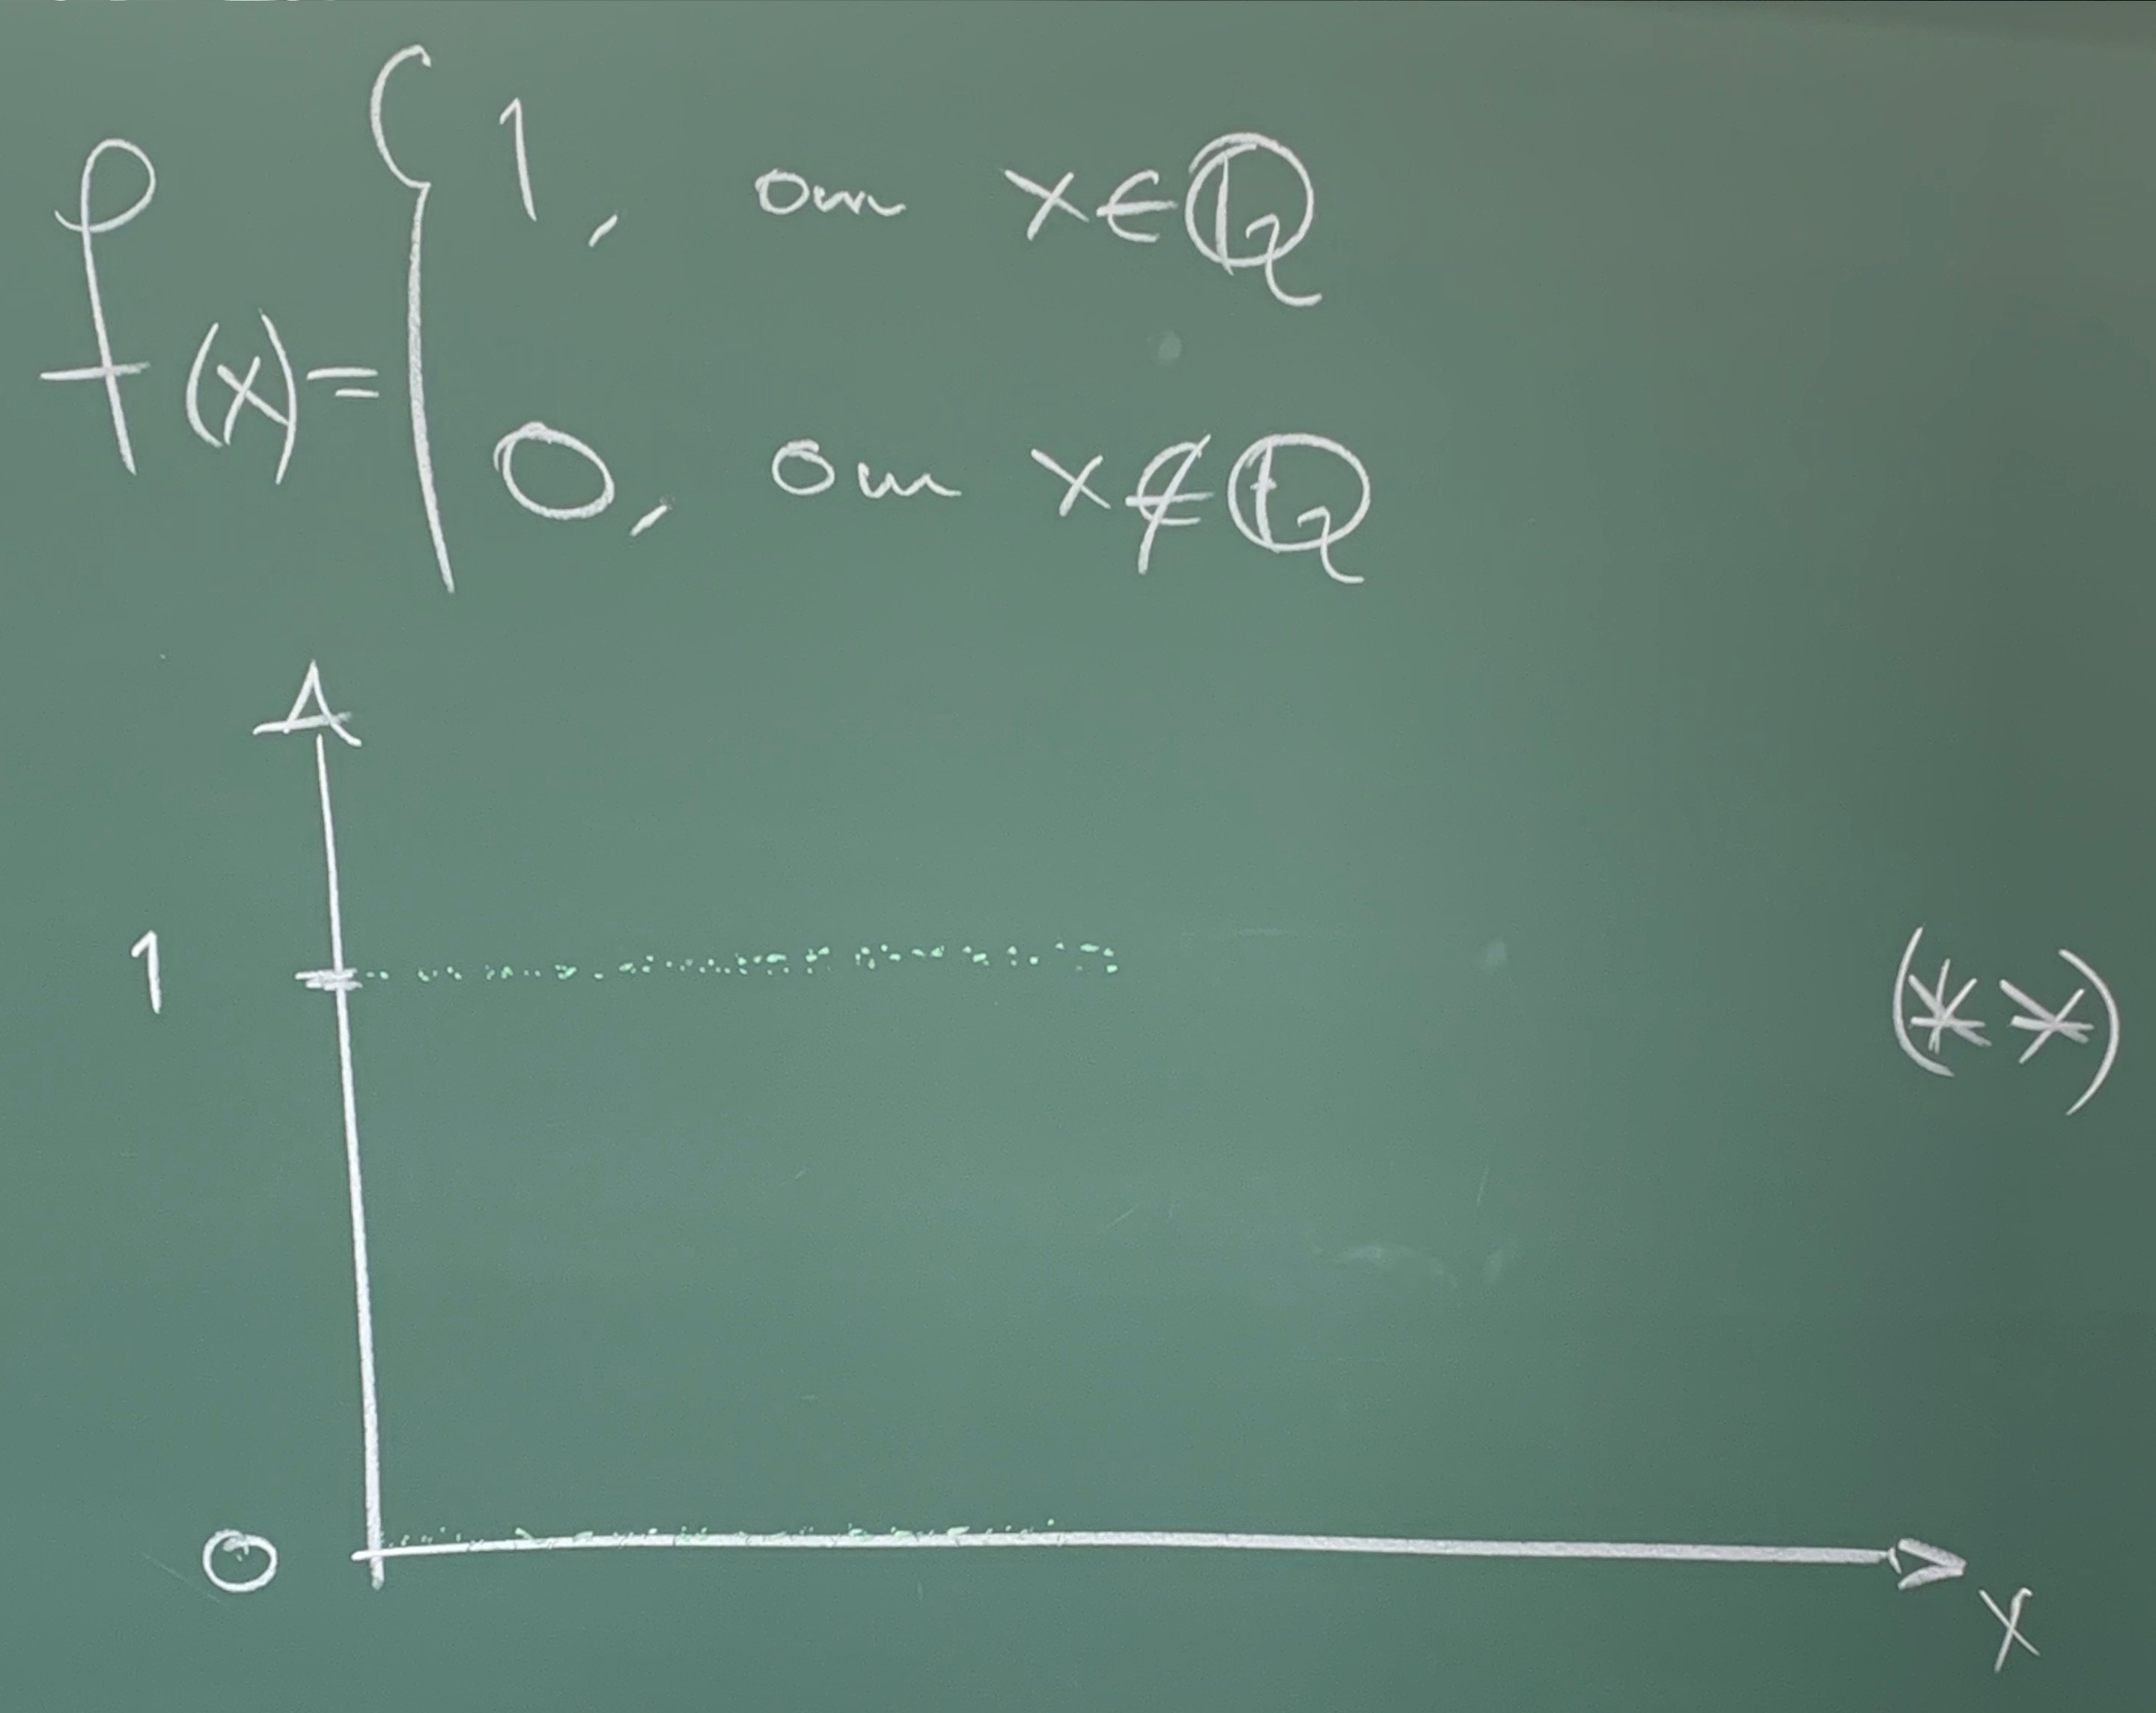
\includegraphics[scale=0.1]{lessons/lesson04/imgs/img01.jpg}

Om man drar en funktion slumpmässigt från mängden av alla funktioner så skulle man nästan säkert dra något i stil med dirichlet funktionen.
Måste därför hitta vettig begränsad klass av funktioner för att kunna hitta meningsfulla matematiska resultat.
En sådan klass är de \underline{kontinuerliga} funktionerna.

\paragraph{Definition} (Kontinuerlig funktion)
Man säger att en funktion $f$ är \underline{kontinuerlig} i punkten $x=c$ (som antas vara en mindre punkt i $D(f)$) om $\lim_{x\to c}f(x)=f(c)$.
Om antingen $\lim_{x\to c}f(x)$ inte existerar \underline{eller} existerar men inte är lika med $f(c)$ säger man att $f$ är \underline{diskontinuerlig} i $x=c$.
Vad betyder detta? Jo, det betyder att "funktionen hänger ihop" i $x=c$.\\
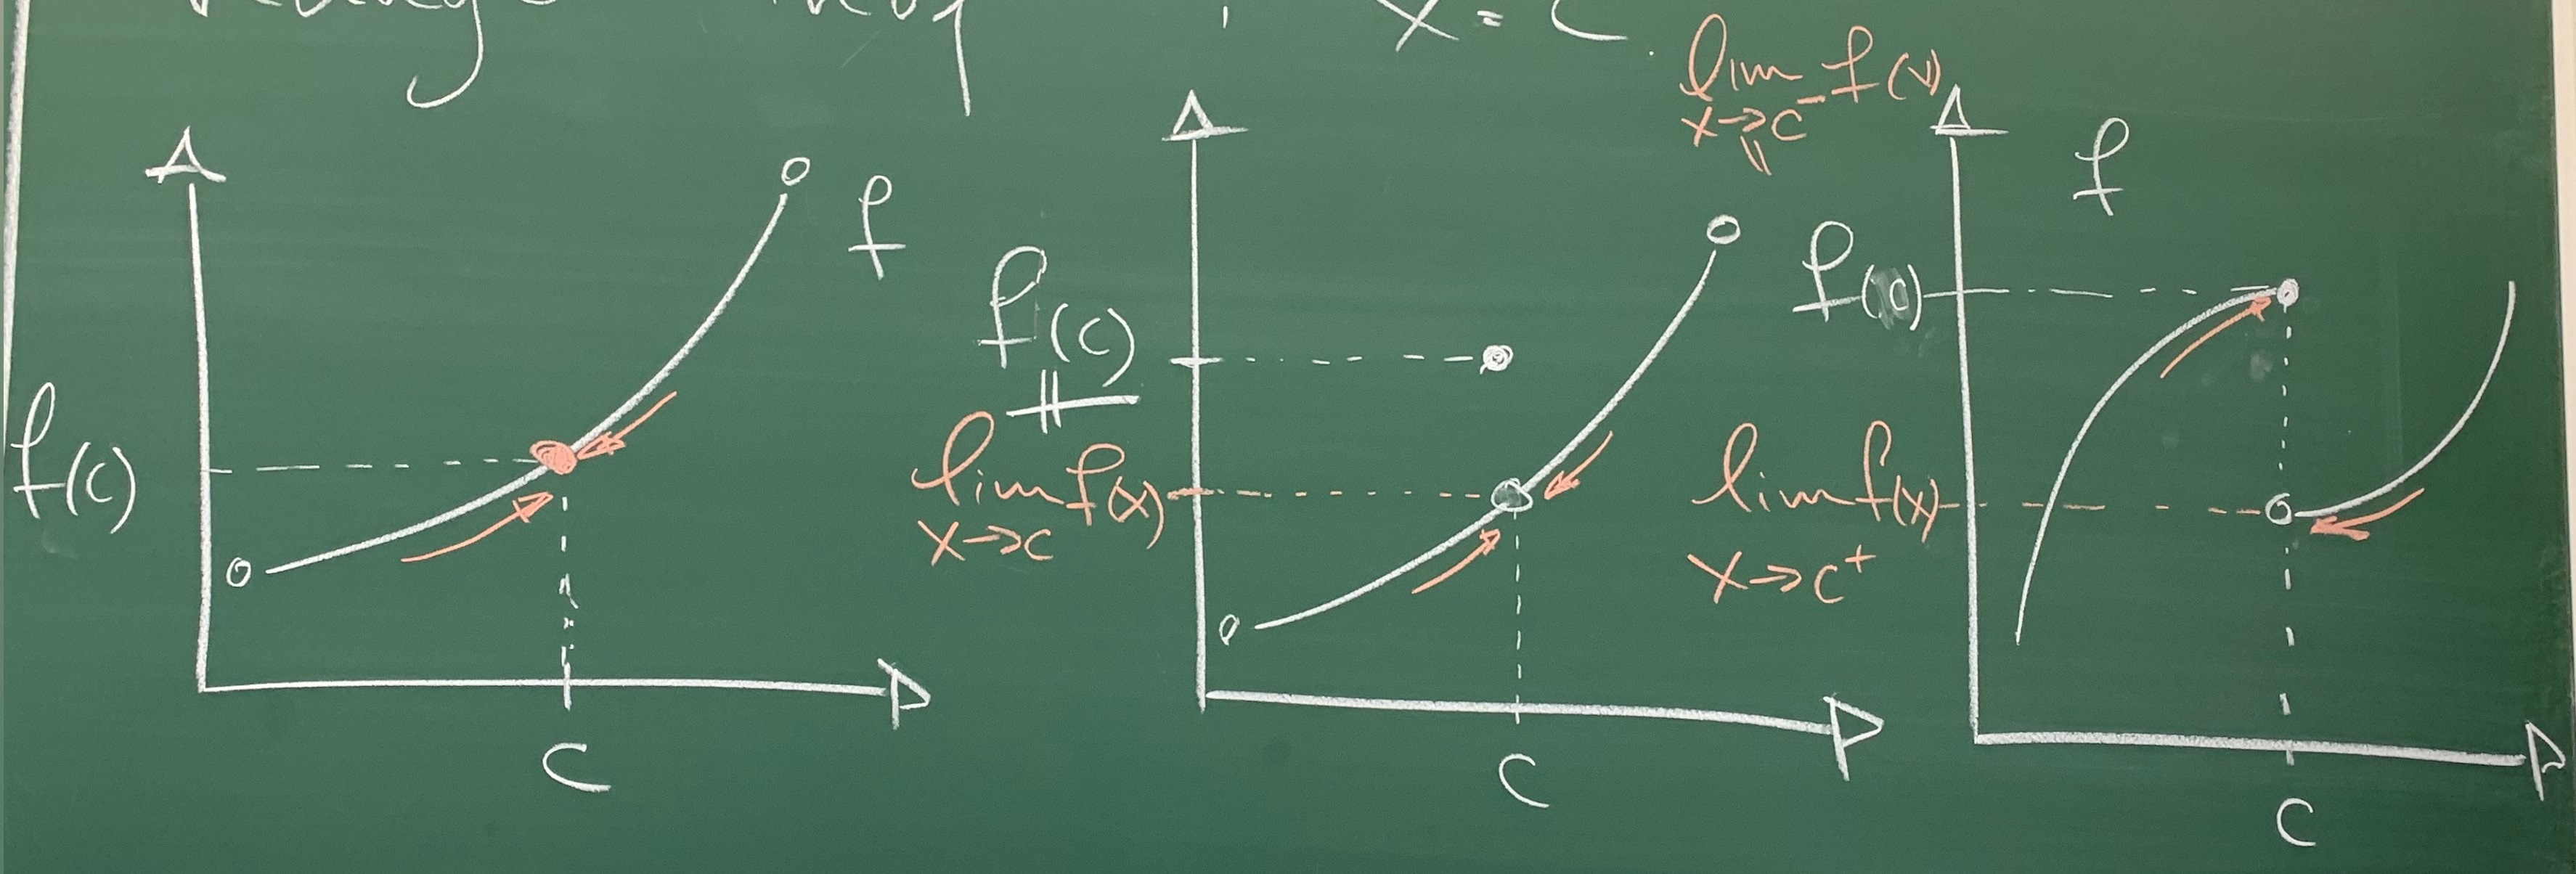
\includegraphics[scale=0.1]{lessons/lesson04/imgs/img02.jpg}\\
Man säger att en funktion $f$ är kontinuerlig på ett helt intervall $I$ om $f$ är kontinuerlig i varje punkt $x\in I$.\\
Hur hanterar man ändpunkterna i $I$? Till exempel om $I=[a,b]$, vad ska gäla för $x\to a$ och $x=b$?
Jo, $f$ ska vara \underline{högerkontinuerlig} i $x=a$ och \underline{vänsterkontinuerlig} i $x=b$.
\begin{itemize}
    \item Man säger att en funktion $f$ är vänsterkontinuerlig i en punkt $x=c$ om $\lim_{x\to c^-}f(x)=f(c)$.
    \item Man säger att en funktion $f$ är högerkontinuerlig i en punkt $x=c$ om $\lim_{x\to c^+}f(x)=f(c)$.
\end{itemize}
Så, $f$ benämns som kontinuerlig i \underline{randpunkter} till ett intervall (till exempel $a$ och $b$ för $[a,b]$) om den är höger- respektive vänsterkontinuerlig.\\
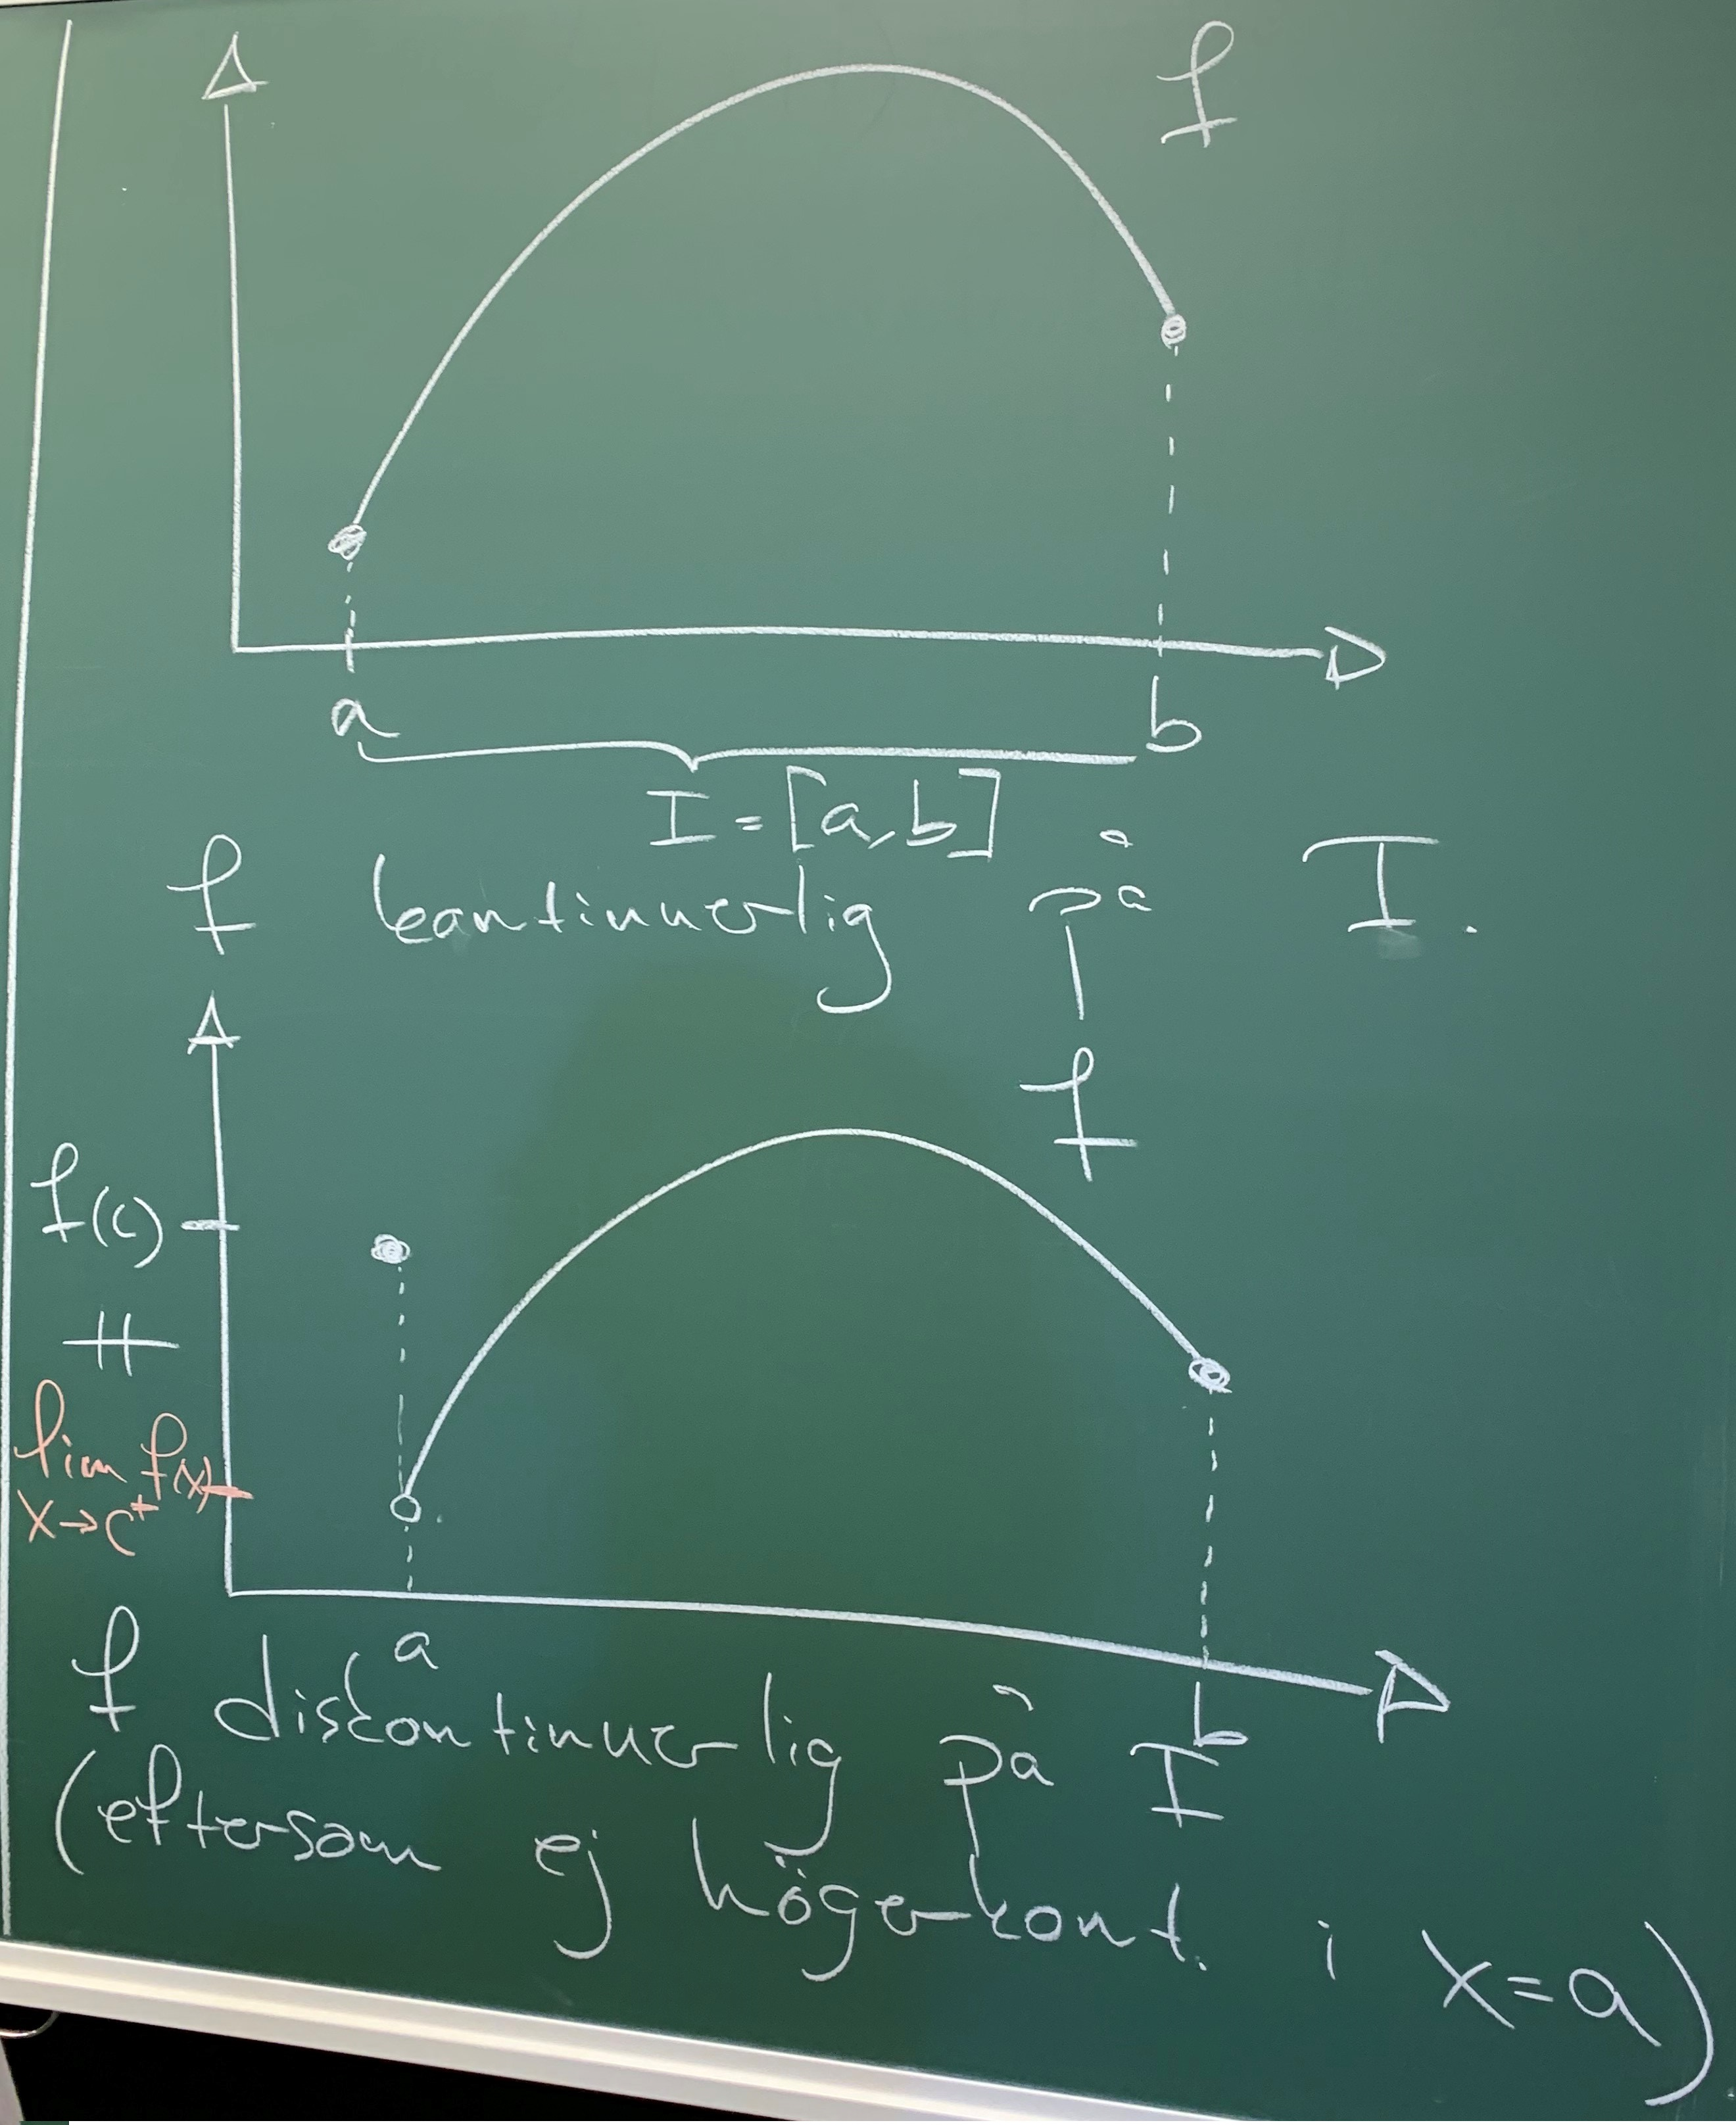
\includegraphics[scale=0.1]{lessons/lesson04/imgs/img03.jpg}\\

\paragraph{Ex (1.4.9)} Beskriv var i sin definitionsmängd som följande funktion är kontinuerlig, vänster- respektive högerkontinuerlig och diskontinuerlig.
\begin{equation*}
    f(x)=\begin{matrix}
        \frac{1}{x^2}\text{, om }x\neq 0 \\
        0\text{, om }x=0
    \end{matrix}
\end{equation*}
\subparagraph*{Lösning}
Försök att skissa funktionen.
\begin{itemize}
    \item funktionen $\frac{1}{x^2}$ är alltid positiv
    \item Om $x$ är \underline{stort} (antingen positivt eller negativt) så är $\frac{1}{x^2}\approx 0^+$
    \item Om $x$ är nära $0$ (antingen positivt eller negativt) så är $\frac{1}{x^2}\approx+\infty$
    \item Uppenbart tt $\frac{1}{x^2}$ är växande på $(-\infty,0)$ och avtagande på $(0,\infty)$.
\end{itemize}
%infoga bild 4
%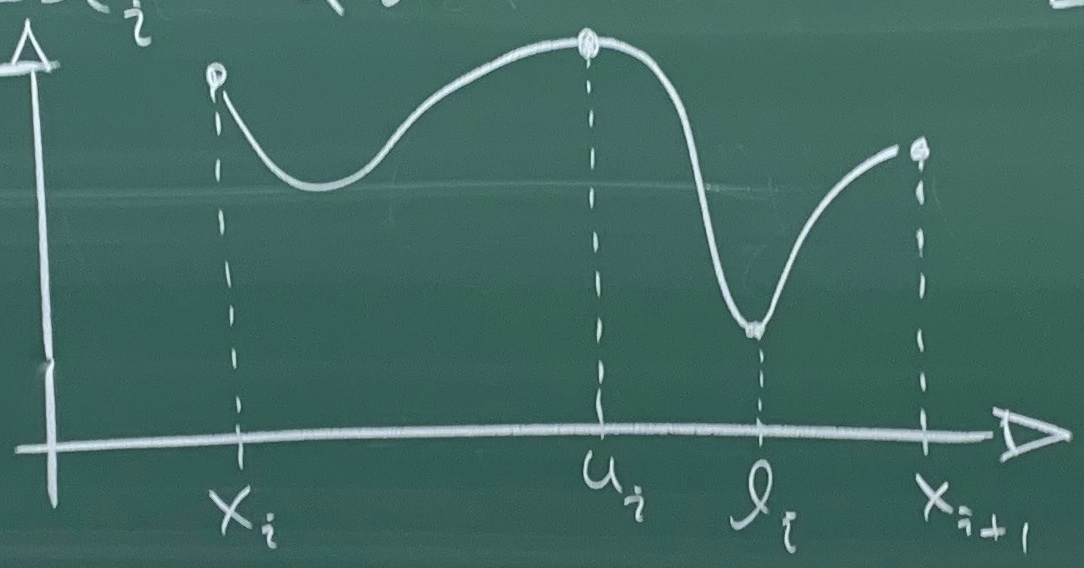
\includegraphics[scale=0.1]{lessons/lesson04/imgs/img04.jpg}\\
Alltså, $f$ är kontinuerlig för alla $x\in\mathbb{R}\setminus \{0\}$ eftersom $\lim_{x\to a}\frac{1}{x^2}=\frac{1}{a^2}=f(x)$ för alla $a\in\mathbb{R}\setminus\{0\}$.
I $x=0$ är $f$ diskontinuerlig eftersom $\lim_{x\to 0}f(x)=\lim_{x\to 0}\frac{1}{x^2}=+\infty$ och $f(0)=0$ och $0\neq\infty\Box$

\paragraph{Ex (1.4.16)} Hur ska man definiera funktionen $f(x)=\frac{x^2-2}{x^4-4}$ i punkten $x=\sqrt{2}$ för att den ska bli kontinuerlig där?
\subparagraph{Lösning} Vad händer i $x=\sqrt{2}$?\\
\begin{equation*}
    f(\sqrt{2})=\frac{\sqrt{2}^2-2}{\sqrt{2}^4-4}=\frac{2-2}{4-4}=\frac{0}{0}\text{???}
\end{equation*}
Vill studera gränsvärdet $\lim_{x\to \sqrt{2}}f(x)$.
\begin{equation*}
    f(x)=\frac{\sqrt{2}^2-2}{\sqrt{2}^4-4}=\frac{x^2-2}{(x^2-2)(x^2+2)}=\frac{1}{x^2+2}\text{ }\overrightarrow{x\to\sqrt{2}}\text{ }\frac{1}{4}
\end{equation*}
Vi ser att $f$ kan naturligt definieras i punkten $x=\sqrt{2}$ även om det inte var uppenbart från början.
Genom att sätta $f(\sqrt{2})=\frac{1}{4}$ så blir funktionen kontinuerlig i $x=\sqrt{2}$, dvs.
$f(x)=
    \begin{matrix}
        \frac{x^2-2}{x^4-4}\text{, om } x\neq\sqrt{2} \\
        \frac{1}{4}\text{, om }x=\sqrt{2}
    \end{matrix}\Box$

\paragraph{Ex (1.5.3)} Beräkna gränsvärdet
\begin{equation*}
    \lim_{x\to 3}\frac{ |5-2x| - |x-2| }{ |x-5| - |3x-7| }
\end{equation*}
\subparagraph{Lösning} Måste reda ut hur det olika absolutbeloppen beter sig i en omgivning av $x=3$.
\begin{equation*}
    |5-2x|=
    \begin{matrix}
        5-2x\text{ om } 5-2x\geq 0 \Leftrightarrow x \leq \frac{5}{2}=2,5 \\
        -(5-2x)\text{ om } 5-2x < 0 \Leftrightarrow x > 2,5
    \end{matrix}
\end{equation*}
\begin{equation*}
    |x-2|=
    \begin{matrix}
        x-2\text{ om } x-2\geq 0 \Leftrightarrow x \geq 2 \\
        -(x-2)\text{ om } x-2 < 0 \Leftrightarrow x <2
    \end{matrix}
\end{equation*}
\begin{equation*}
    |x-5|=
    \begin{matrix}
        x-5\text{ om } x-5\geq 0 \Leftrightarrow x \geq 5 \\
        -(x-5)\text{ om } x-5 < 0 \Leftrightarrow x < 5
    \end{matrix}
\end{equation*}
\begin{equation*}
    |3x-7|=
    \begin{matrix}
        3x-7\text{ om } 3x-7 \geq 0 \Leftrightarrow x\geq \frac{7}{3}\approx 2,33 \\
        -(3x-7)\text{ om } 3x-7 < 0 \Leftrightarrow x < 2,33
    \end{matrix}
\end{equation*}
Vi kan alltså skriva gränsvärdet som:
\begin{equation*}
    \lim_{x\to 3}\frac{2x-5-x+2}{5-x-3x+7}=\lim_{x\to 3}\frac{x-3}{-4x+12}=\lim_{x\to 3}\frac{x-3}{-4(x-3)}=\frac{1}{4}\Box
\end{equation*}